% TEMPLATE for Usenix papers, specifically to meet requirements of
%  USENIX '05
% originally a template for producing IEEE-format articles using LaTeX.
%   written by Matthew Ward, CS Department, Worcester Polytechnic Institute.
% adapted by David Beazley for his excellent SWIG paper in Proceedings,
%   Tcl 96
% turned into a smartass generic template by De Clarke, with thanks to
%   both the above pioneers
% use at your own risk.  Complaints to /dev/null.
% make it two column with no page numbering, default is 10 point

% Munged by Fred Douglis <douglis@research.att.com> 10/97 to separate
% the .sty file from the LaTeX source template, so that people can
% more easily include the .sty file into an existing document.  Also
% changed to more closely follow the style guidelines as represented
% by the Word sample file. 

% Note that since 2010, USENIX does not require endnotes. If you want
% foot of page notes, don't include the endnotes package in the 
% usepackage command, below.

% This version uses the latex2e styles, not the very ancient 2.09 stuff.
\documentclass[letterpaper,twocolumn,10pt]{article}
\usepackage{usenix,epsfig,endnotes,graphicx}
\usepackage{epstopdf, color}
\usepackage{enumitem}
\setlist[enumerate]{itemsep=0mm}
% \DeclareGraphicsExtensions{.eps}

\usepackage{listings}

\lstset{
    language=python,
    numbers=left,
    tabsize=2,
    showstringspaces=false,
    showspaces=false,
    numberstyle=\footnotesize, %tiny, footnotesize
    xleftmargin=1em,
    frame=leftline, %lines
    resetmargins=true,
}


\begin{document}

%don't want date printed
\date{}

%make title bold and 14 pt font (Latex default is non-bold, 16 pt)

\title{\Large \bf BugBox : A Vulnerability Corpus for PHP Web Applications}


%for single author (just remove % characters)
\author{
{\rm Gary Nilson}\\
Computer Science Department\\University of Maryland
\and
{\rm Kent Wills}\\
Computer Science Department\\University of Maryland
\and
{\rm Jeff Stuckman}\\
Computer Science Department\\University of Maryland
\and
{\rm Jim Purtilo}\\
Computer Science Department\\University of Maryland
% copy the following lines to add more authors
% \and
% {\rm Name}\\
%Name Institution
} % end author

\maketitle

% Use the following at camera-ready time to suppress page numbers.
% Comment it out when you first submit the paper for review.
\thispagestyle{empty}

%Orphaned sentences
%  Furthermore, the framework capability is streamlined through the thorough use of abstraction and encapsulation making the management of the application, environment, and exploitation in BugBox. \\
% The study of identifying vulnerability points and their representations is often refered to as \emph{vulnerability localization}[ref].\\

%[REF A database of computer attacks for the evaluations of IDSes]
%Generating Realistic traffic... DARPA IDS (long ref).. 300 attacks.. 32 types.. 7 different scenarios
%Realistic variance of methods used by the attacker..

%Some suggestions from Jim: 
%Consequences of use: good for many references.
%Evaluation
%Why is this hard.
%Why have others not done it yet.
%Abstract:
%What makes it ours?
 

\subsection*{Abstract}
\textit{
PHP Web Applications are a rich source of vulnerabilities due to their high exposure, diversity, and popularity. Accordingly, they are ideal specimens for empirical vulnerability research. There are not, however, publicly available resources of vulnerabilities that are both robust and practical to use. BugBox is an open-source corpus and framework for PHP web application vulnerabilities created to fill this void, and in doing so encourage greater quality security research. In this paper we describe Bug Box as a mechanism that encourages the distribution of vulnerability data and further supports research in developing vulnerability definition representations, testing intrusion detection systems, testing static analysis tools, and separately as a tool for training purposes.  
}

\section{Introduction}
PHP Web applications are subject to a rich variety of exploit types, such as cross-site scripting (XSS), cross-site request forgery (CSRF), buffer overflow, and SQL injection.  A recent study by White Hat Security~\cite{WhiteHat:2010:Online} analyzed seven web application languages: ASP, ASPX, CFM (Cold Fusion Markup), DO (Struts), JSP, PHP, and PL (Perl) showing that PHP, while having the smallest attack surface in their tests, produced one of the highest average number of serious vulnerabilities per website.  This variety of exploits in PHP and other languages is logged extensively in popular exploit databases such as the National Vulnerability Database (NVD), Open Source Vulnerability Database (OSVDB), Common Vulnerability and Exposures Database (CVE), or the Exploit Database (EDB).\par

While many of these databases are easy to access and disclose the details of the vulnerability and/or exploit, they do not provide a collection of structured vulnerable code, a corpus, that can support statistical analysis and hypothesis testing.  The pursuit for such a corpus was driven through prior research, in developing attack surface metrics~\cite{Stuckman:2012:CAA:2372225.2372229} and evaluating intrusion prevention systems~\cite{Stuckman:2011:TEW:2195220.2195671}, and is furthered through our continued research in dynamic decentralized intrusion detection.  Furthermore, a corpus can facilitate a variety of activities of interest to the security community including evaluating static analysis tools~\cite{Zitser:2004:TSA:1041685.1029911}, penetration testing and training security teams on vulnerability injection~\cite{4725309}, and analyzing open source web applications~\cite{DBLP:journals/ese/HuynhM10}.  \par

BugBox is a framework  that streamlines the collection and sharing of vulnerability data and facilitates cyber security experiments.  This mechanism allows users to identify a vulnerability in a web application, quickly develop an exploit script, and collect execution traces of vulnerability data, all of which can be easily packaged and distributed to the community.
 
\section {The Structure and Contents of a Corpus}

\subsection{Application Packaging and {\tt chroot} Environment}

A key responsibility of the framework is to manage packaged vulnerable applications in an automated way. This includes doing tasks needed to setup the operating system, web server, PHP interpreter, and the application itself. Since every application has it's own system requirements, the configuration is joined with the application itself within {\bf Target} modules existing in the corpus. It is the job of the {\bf Engine} to then match exploits with targets and actualy perform setup, configuration, and teardown work. The Engine will actually mount the web application's folders within an associated chroot jail, 

We use Linux {\tt chroot} jails as the host environments to support target applications with varying system requirements.  The Engine stages the application within the {\tt chroot} environment provides locality, reproducibility, and stability. The following properties are reasons supporting the use of {\tt chroot} jails as the target environments:\par
{\bf The web application remains local}.  Many applications, such as WordPress, have a MYSQL back end.  If we were to host the application on a different server or VM we would have to ensure that the MYSQL database is properly setup each time.  With the {\tt chroot} environment, the process is simplified. We keep a MYSQL database outside of the {\tt chroot} Jail in order to facilitate web application configuration. \par
{\bf Current tests are independent from future tests}.  We load a clean application into the {\tt chroot} jail every time we wish to run a new test.  This ensures that there is no corruption of the original web application and provides reproducible results when testing.\par
{\bf The web application cannot contaminate our testing environment}.  If a web application crashes due to the malicious script, we can ensure that it does not crash our corpus environment.  In the worst case the {\tt chroot} becomes corrupt for which we can treat in an isolated scenario that does not have un-intended side effects in our testing environment.\par
{\bf The web application will never be contaminated}.  We store a separate backup in order to verify that the selenium scripts did not modify the Web Application in any way.  If the Web Application is corrupt, then we simply copy the web application from the backup folder to the package folder.  Future implementations will store only the md5 hash of the program on the corpus server and the backups on an external server.  This will allow for a quick comparison followed by a remote copy for mismatched hashes.  This separation will ensure that backups will never be corrupted through use of the corpus and expedite checking.\par
{\bf Applications with different OS environments can be run}.  If an application was built for Debian 6 as opposed to Debian 4, we can setup a {\tt chroot} environment that has support for that specific OS.  This gives us the flexibility to test the web application in whatever OS environment we choose.\par
{\bf Scalability}.  In order to create a system that can handle a growing amount of vulnerabilities that are independent from one another, we represent an exploit on an application through exploit scripts, as noted in the Framework section.  Exploit scripts allow us to perform operations on web applications without fear of working in an un-intended, compromised environment.  Scalability is critical because we ultimately want to do mass, automated experiments in tandem. 
{\bf Introspection} Since the {\tt chroot} environments exist on the host machine as simple directories, it is trivial to write scripts for managing the environment. This property allows for easy management of web applications, simple maintenance using incremental backups, and provides for other paths of research such as system taint analysis.

\subsection{Development}

To add a new entry to the corpus one has to create two to four main entities. Writing an exploit, and generating an execution trace are required, and depending on the target application, one may have to define a new target module, and/or in rare cases, create a new target environment. However, often there are multiple exploits for a given target application, so it is not always necessary to create a new one. And because PHP web applications do not tend to have a large range of system dependencies, the majority of targets require at most a handful of different OS environments. \par
The format of a BugBox exploit should look familiar to anyone who has worked with the Metasploit framework. The exploit must contain a procedure for attacking a specific application, and potentially one or two others for doing pre-exploitation checks of the target, and post exploitation cleanup of the target's environment (for example, removing any files that were uploaded to a web server). \par
The execution trace is generated using XDebug to capture the application's state throughout exploitation. XDebug is a feature-rich PHP extension which provides debugging and profiling capabilities.  For our purposes, we use it to capture traces through setting its global environment auto-trace variable. XDebug is instructed to collect the execution traces during this process, and finally the corpus engine collects and organizes them on a per-session basis. Currently we toggle this on a session basis, but plan for support to be manage the trace collection through the setting of cookies while the script is being executed. \par
The target module represents web applications in their vulnerable state. To add a new vulnerability to the corpus, we first select an application and determine whether the package is defined in the corpus, and proceed to create a target module if necessary. Although we focus primarily on open source applications, it is sometimes hard to obtain vulnerable the versions of an application. This step may involve hunting down patches in a mailing list or searching through the branches of a source repository. We perform a manual execution of the exploit to verify that we understand the scope of the exploit, from which we proceed to write a script for the exploit so that the process will integrated into the corpus. Finally, we collect the trace of the program while our script is being executed and add it to our corpus. Similarly, a target environment (the OS) includes the entire set of dependencies of the web application, such as PHP version, or web-server.\par


\subsection{Methods for Localization}

A key question across many applications of empirical vulnerability research is how to represent which functionality, or piece of code accounts for the vulnerable condition in a program. In studying this problem, referred to as \emph{vulnerability localization}, it is important to have a large quantity of structured data to test hypotheses. The desired properties of this structured data may vary by line of study, but in the BugBox framework the primary method proposed for capturing code vulnerabilities is through the collection of execution traces. We accomplish this task by collecting execution traces during exploitation using XDebug, and then manually highlight the program paths relevant to the vulnerability.\par 
Line-based, run-based, and trace-based approaches are all effective types of vulnerability localization definitions. A line-based~\cite{4630094} approach for vulnerability collection uses line numbers represented in program patches to identify the location of the vulnerabilities.  However, there are many ways to fix a vulnerability and a patch represents only one of these ways or may represent irrelevant changes.  A run-based~\cite{Song:2008:BNA:1496255.1496257} approach creates vulnerability signatures from intermediate byte code. The drawback to this approach is that it does not isolate the lines of source code that represents the vulnerability. Execution traces, on the other hand, where traces are classified as \emph{potentially exploitative} or \emph{non-exploitative} allow for great flexibility matching programs against vulnerability signatures. A drawback to this approach, is that to increase the accuracy of the data, currently one must manually refine the traces.   \par






\section {An Application and Framework}

\subsection {An Example Execution of BugBox}

The following Python scripts illustrate two use-cases for the BugBox framework. Both of these examples show ways to make use of vulnerability meta-data to run different experiments. In the first example, all XSS vulnerabilities existing in the the corpus are sequentially invoked, and execution traces are collected for analysis:

\begin{minipage}{\textwidth}
{\tt \footnotesize

\begin{lstlisting}
 import config
 from framework import Query, Engine
 
 for Exploit in Query().get_by_type('XSS'):
    engine = Engine(Exploit(), config)
    engine.startup()
    engine.xdebug_autotrace_on()
    engine.exploit()
    engine.xdebug_autotrace_off()
    engine.shutdown()
\end{lstlisting}
}
\end{minipage}

%\caption{Example 1:}

Here, instead of collecting traces for all vulnerabilities of the same type, we are interested in running all exploits across all versions of a given application:

\begin{minipage}{\textwidth}
{\tt \footnotesize
\begin{lstlisting}
import config
from framework import Query, Engine

for Exploit 
    in Query().get_by_re('Target', 
                         'Wordpress.*"):
    engine = Engine(Exploit(), config)
    engine.startup()
    engine.xdebug_autotrace_on()
    engine.exploit()
    engine.xdebug_autotrace_on()
    engine.shutdown()
\end{lstlisting}
}
\end{minipage}
%\caption{Example 2:}

For simple jobs where the focus of study is a single vulnerability or vulnerable application, the run-time management of a single corpus entry can be done from the command-line. The most basic commands are provided in the \emph{bbmanage.py} utility with the following options:

%{\tt \small
{\tt \footnotesize
\begin{verbatim}
Usage: ./bbmanage.py [command] <options>
    Commands:   Options:
    list        <exploits | targets | 
                 types    | running>
    info        <exploit_name>
    start       <exploit_name>
    exploit     <exploit_name <display>>
    stop        <exploit_name>
    trace_on    <exploit_name>
    trace_off   <exploit_name>
    autorun     <exploit_name>
\end{verbatim}
}

The process of setting up an OS environment, configuring the target application, interacting with the PHP debugger, and all post-job cleanup occur behind the scenes in the BugBox framework. Any of these tasks would have taken hours to accomplish using our previous approach, which was based on manually managing various virtual machine snapshots. Using Python as a layer of abstraction above the OS, target application, and exploits, it is now possible to easily automate research tasks. The following sections give an overview of the system design that makes this abstraction possible.

\subsection{Framework}

%{\bf SeleniumDriver}, {\bf Exploit},
Figure 1 illustrates the structure of the corpus, with boxes and arrows showing lines of control or communication. The framework breaks down logically into the following five components: {\bf Host Environment} (currently the Virtual Machine), {\bf Engine}, {\bf Target Environment}, {\bf Target}, and {\bf Exploit}. The diagram shows that the corpus is composed of any number of exploits, {\tt chroot} jails, target applications, and associated target plugins, that exploits and {\tt chroot} jails are under control of the vulnerability engine, the exploits interact directly with the target application (during exploitation) both through the Selenium Server and directly using libraries such as \emph{urllib}, all databases associates with the target applications are hosted directly on the host environment, and the database server is under control of the vulnerability engine.\par
Except for the host environment, each of the five major components are represented directly in BugBox as either a Python module or a package. The design is intended to make it practical to manage a large database of exploits, along with their target environments. For each exploit, all relevant details of a vulnerability are maintained for the researcher. A given corpus entry we include the software in which a vulnerability exists, the configuration of the software in it's vulnerable state, exploit code that will trigger the security breach, and any relevant meta-data.\par

\begin{figure}[!tp]
\begin{center}
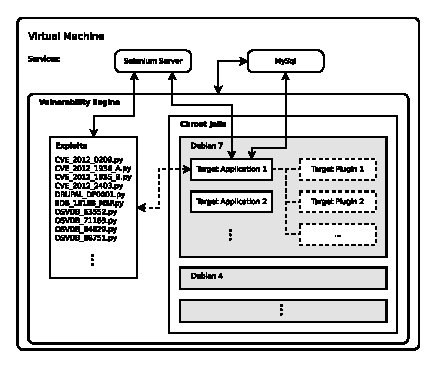
\includegraphics[scale=1.17]{system_diagram.eps}
\end{center}
\caption{System Diagram}
\end{figure}


\subsubsection{Engine}
The {\bf Engine} drives the environment setup, tear-down, and exploitation process. The engine was created to abstract away details so that researchers can easily run exploit scripts without having to worry about getting the target application running every time. \par
The vulnerability engine controls the actions of a given exploit, and ensures that the proper target environment, application, and application plugins are properly setup in the {\tt chroot} environment. The role of the engine is illustrated in the two use-cases. For example, following relevant lines in Use-Case 1:
\begin{description}
  \item[Line 5] {\tt \footnotesize    engine = Engine(Exploit(), config)} \\ A new engine instance is constructed with an exploit instance and system configuration as arguments.
  \item[Line 6] {\tt \footnotesize     engine.startup()} \\The engine creates a {\tt chroot} environment on the host system to which the target application is copied and the pertinent MYSQL databases are established. The setup of the environment is determined by the 'Target' attribute in the exploit instance. 
  \item[Lines 7 \& 9] {\tt \footnotesize engine.xdebug\_autotrace\_on()\\ engine.xdebug\_autotrace\_on()}\\The engine can modify the state of the trace collection in X\_Debug to ensure that we collect only the trace pertinent to the exploitation.
  \item[Line 10] {\tt \footnotesize engine.shutdown()}\\Cleanup unmounts the {\tt chroot} environment and returns the corpus environment back to an un-altered state.
\end{description}



%\begin{figure}[!tp]
%\begin{center}
%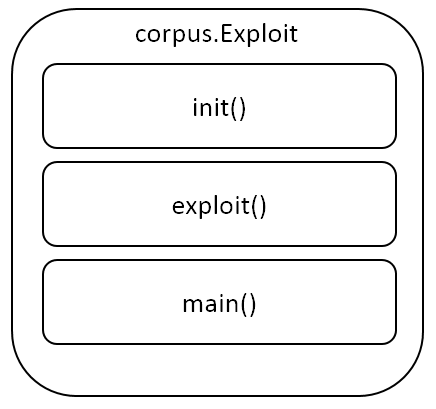
\includegraphics[scale=.5]{Corpus_Exploit.PNG}
%\end{center}
%\caption{Exploit Structure}
%\end{figure}


\subsubsection{Targets}
   The {\bf Target} module controls all the application targets that the exploits may be applied to.  More specifically, this represents web applications such as WordPress, SimplePHPAgenda, etc. A copy of the target program with a typical configuration, is always loaded before any exploit script is run.  Init scripts are written per application to provide the {\bf Engine} with the proper details for the setup, for example:

\begin{minipage}{\textwidth}
{\tt \footnotesize
%\begin{verbatim}
\begin{lstlisting}
name = "Wordpress 3.3.1"
application_dir_mapping = ...
     [get_path("application"), "/var/www"]
database_filename = get_path("database.sql")
database_name = "wordpress_3_3_1_A"
chroot_environment = "Debian7"
\end{lstlisting}
%\end{verbatim}
} 
\end{minipage}


Some large web applications, such as WordPress, have many plugins that in themselves, have vulnerabilities. Therefore {\bf Target} modules also allow for the inclusion of plugins in the exploit framework.Both targets, and target plugins are resolved against the exploit attributes by the Engine during the setup process. 


\subsubsection{Exploit}
The {\bf Exploit} class is the superclass for each exploit in the corpus, defining interfaces and attributes that the engine uses to manage the environment and exploitation. The structure of Exploit is designed so that exploits can be written as a concise code statement. Each exploit is simply a subclass of Exploit residing in it's own Python file in which all actions taken by the exploit are clearly visible. In addition, a Query module is provided that will return a set of Exploit instances based on matching against the meta-data specified in the exploit (as shown in the use-cases).\par

This separation accomplishes a step-like approach for getting involved with the corpus, where developing exploits for the corpus is more approachable and quick for novice programmers that wants to contribute and a robust framework that can be understood incrementally for larger contributions to the framework.\par
 
This template ensures that the selenium driver is properly initialized bound to the exploit and makes sure that an exploit script has been defined as well as defines any specific actions on tear-down.\par

The exploit module is annotated by it's attribute dictionary. This structure is inspired by the exploit class from the Metasploit~\cite{MetaSploit:2012:Online} module. In it we declare the name, description, references, target, type and wiki page for the exploit by the attributes dictionary.  The name is the technical name specified in one of the online databases of exploits and vulnerabilities mentioned earlier in the paper.  The description is a brief statement of what the exploit is supposed to do, because the name is typically not descriptive enough for a person to understand what type of exploit is being applied.  The Target is the web application target that is being used for the exploit.  The type is the type of exploit being conducted.  The VulWikiPage is the wiki page setup for an author to place auxiliary information about the exploit or script.  The following represents the attributes entries for an example XSS exploit:\\


{\tt \small
\begin{tabular} { l l }
\noindent{\bf Name}&CVE\_2012\_2403\\
{\bf Description}&Creates a post containing a\\& XSS payload.\\
{\bf References}&CVE 2012-2403, OSVDB 81463 \\
{\bf Target}&Wordpress 3.3.1\\
{\bf Type}&XSS\\
{\bf VulWikiPage}&WIKIHOST/CVE-2012-2403
\end{tabular}
}

Here is an example body of an exploit procedure used for the simplest of XSS attacks.  The entire exploit consists only of instantiating the selenium driver and submitting a post on the WordPress site with the payload: 

\begin{minipage}{\textwidth}
{\tt \footnotesize
%\begin{verbatim}
\begin{lstlisting}
payload = "<a href=\"#\" title=\"XSS http:" \
          "//example.com/onmouseover=eval(" \
          "unescape(/%61%6c%65%72%74%28%31" \
          "%29%3b%61%6c%65%72%74%28%32%29%" \
          "3b%61%6c%65%72%74%28%33%29%3b/." \
          "source))//\">XSS</a>"

driver = self.create_selenium_driver()

driver.get("http://localhost/wordpress/?p=1")
get = driver.find_element_by_id
get("author").send_keys("selenium script")
get("email").send_keys("selenium@python.org")
get("url").send_keys("www.python.org")
get("comment").send_keys(payload)
get("submit").click()
\end{lstlisting}
%\end{verbatim}
}
\end{minipage}

\section {On-Going Development and Conclusion}

\subsection{Security Demonstrations}

Exploits mostly interact with the world through a {\bf SeleniumDriver} class that serves as a wrapper to Selenium's Firefox web driver. This allows the framework to leverage Selenium's powerful browser automation. Selenium integrates nicely with the framework using stable and well-documented Python bindings, providing demonstration/visualization capabilities, JavaScript support, and easy interaction with HTML objects.\par
This wrapper class allows the exploit writer to choose whether to display the Firefox browser during exploitation. This feature has proven very useful for debugging exploits, and has lead to quicker turn-around in the exploit development. With the Selenium Driver, one can also orchestrate demonstrations to teach others the principles behind web vulnerabilities.  A setup could entail showing a live feed of tcpdump and the Apache logs on one screen, while in real-time one Firefox process shows the actions taken by an attacker posting a malicious script on a forum, after which the session for an unsuspecting admin in an adjacent Firefox process shows the activation of a CSRF exploit. 

\subsection{On-going Development}
  Future development on the framework will include features for controlling trace collection through cookie manipulation via XDebug. This will reduce the collection of insignificant interactions and provide a more refined break-down of the exploitation process since traces can be grouped by HTML request. In order to achieve this, we may have to explore the possibility of forcing the exploit writer to use a single communication interface, instead of the Selenium/cookielib/urllib combination in the current approach. This may be necessary in order to cleanly interact with XDebug with appropriate cookies set on a per-request basis (especially when modules other than Selenium are used for communication).\par
For each exploit currently in the corpus, there is no standard for the payload used in the attack. Since many studies may be sensitive to the payload type and encoding, it makes sense to provide the researcher with fine-grained control over this property. The Metasploit Framework has a very robust system for managing exploits along with their payloads and encodings, and can be a model for implementing this.

\subsection{Lessons Learned}

Some research projects conducted in our software engineering group at the University of Maryland are centered around collection of metrics data for vulnerabilities.  Since we were unable to find a corpus that suited our needs, we started to build an in-house corpus.  Originally our corpus architecture was a VM based. \par
The idea was to be able to mount web application targets onto VMs.  We had a similar idea in th sense that the VM's could be setup and brought down, saving the current state that they were in.  Once the application was mounted, we performed an exploit manually and saved a snapshot of the VM instance.  All exploits applied to "tainted" applications, so we had to be careful that one exploit did not interfere with another.  We hired summer students to create exploits and save new snapshots, from which we had them report their progress on the wiki we had built.\par
We found that because the process was not sufficiently documented, it was harder to verify that the exploit was executed in the correct manner.  Many times pages that were logged as exploited, did not show the representation of the exploit. Furthermore it was not possible to perform automated query-able tests for the collection of exploits.\par

\subsection{Availability}

BugBox is designed to work on the Debian GNU/Linux and compatible distributions.  It is distributed both as as a self-contained virtual machine, and as a package that can be installed on an existing system. The machine must have sufficient storage (roughly 4 GB per OS environment, and 2 GB for the application, engine, and exploit sources), with access rights to use run Linux {\tt chroot} jails.  Dependencies for the BugBox host system include MySQL, Selenium Server, debootstrap, the Advanced Packaging Tool (APT.), and any minimum hardware requirements for running the target web applications.\par

Community contributions will be key to building a corpus of sufficient size. Therefore, all code and data is licensed by the University of Maryland under the GPL v3, so that contributions and modifications will remain Open Source. In addition, we maintain a vulnerability wiki detailing the entries in the corpus, and a web-interface for the git repository that where the code is managed. Collaboration will be coordinated through the issue tracking system on the website, with git, and through the mailing list. \par

The corpus can be downloaded at:

\begin{center}
{\tt  http://bugbox.cs.umd.edu}
\end{center}

Or can be checked out from the git repository using:

\begin{center}
{\tt git clone bugbox.cs.umd.edu/bbframework.git}
\end{center}

Details on the existing corpus entries can be found on our wiki at:

\begin{center}
{\tt http://www.vulnwiki.com}
\end{center}

\section*{Acknowledgments}

The authors thank the United States Office of Naval Research for its support for this research under contract N000141210147.


While there is not a general definition of corpus quality, we choose to define quality in the statistical sense as a representative sample.  Deriving the following criteria for establishing the suitability of our corpus: type of the samples, quantity of the samples, diversity of the samples, and testing reproducibility to retrieve the samples.



{\footnotesize \bibliographystyle{acm}
\bibliography{ref}}

\end{document}







